% 五号字体,开明式标点处理,不设置默认字体
\documentclass[UTF8,12pt,punct=kaiming,fontset=none]{ctexart}
\usepackage{fontspec}  % 字体
\usepackage{subcaption}  % 节标题
\usepackage[colorlinks=true, linkcolor=magenta, citecolor=magenta, urlcolor=magenta]{hyperref}  % 超链接
\usepackage{geometry}  % 页面布局
\usepackage{fancyhdr}  % 页眉页脚
\usepackage{titlesec}  % 标题
\usepackage{caption}  % 图表标题
\usepackage{floatrow}  % 图表排版
\usepackage{graphicx}  % 图片路径
\usepackage{enumitem}  % 列表

% 图片路径
\graphicspath{{figures/}}

% 字体
\setCJKmainfont{Source Han Serif SC}
\setCJKsansfont{Source Han Sans SC}
\setmainfont{CMU Serif}

% 布局
\geometry{a4paper,left=2cm,right=2cm,top=2.5cm,bottom=2.5cm}
\setlength{\headheight}{25pt}

% 图表标题
\DeclareCaptionFont{captionfont}{\small}
\captionsetup{font=captionfont}
\floatsetup{style=plaintop}

% 页眉页脚
\pagenumbering{arabic}
\pagestyle{fancy}
\fancyhead[L]{· \hspace{0.1cm} \thepage \hspace{0.1cm} ·}
\fancyhead[C]{红 \hspace{0.1cm} 石 \hspace{0.1cm} 数 \hspace{0.1cm} 电 \hspace{0.1cm} 评 \hspace{0.1cm} 论\\\scriptsize{Review of Redstonic Digital Circuit}}
\fancyhead[R]{第1期\\\scriptsize{2022年2月}}
\fancyfoot[L,C,R]{}

% 首页页码
\input{页码.inc}

% 标题
\title{\vspace{-1.5cm}一种物品缓存器方案\vspace{-0.5cm}}
\author{@柠喵喵喵\thanks{作者的B站用户名:柠喵喵喵}}
\date{}

% 参考文献标注
\newcommand*{\upcite}[1]{
    \textsuperscript{\cite{#1}}
}
\setlist{nosep}

\begin{document}
\pdfbookmark{一种物品缓存器方案}{\thepage}  % 书签
\hypersetup{bookmarksdepth=-1}  % 禁止后续书签
\maketitle
\thispagestyle{fancy}  % 首页页眉页脚
\vspace{-0.7cm}

% 节标题格式
\titleformat{\section}[hang]{\large\sffamily\bfseries}{\textmd{\thesection}}{0.5cm}{}
\titlespacing{\section}{0cm}{0.5ex}{0.2ex}
\titleformat{\subsection}[hang]{\normalsize\sffamily}{\textmd{\thesubsection}}{0.5cm}{}
\titlespacing{\subsection}{0cm}{0.5ex}{0.2ex}
\setcounter{section}{0}

本文展示一种物品缓存器方案,实现了将少量多次输入的物品流缓存后一次性输出。尽管目前还没有明确的应用,但我们认为这一设计是有趣且优雅的。其工作原理如图\ref{fig:1}所示。

具体工作流程为:首先锁定漏斗,当缓存容器中的物品逐渐增多,比较器检测到的信号达到一定强度时,解锁漏斗,一次性将容器清空,之后再次锁定漏斗,进行下一轮工作。

\begin{figure}[h]
    \centering
    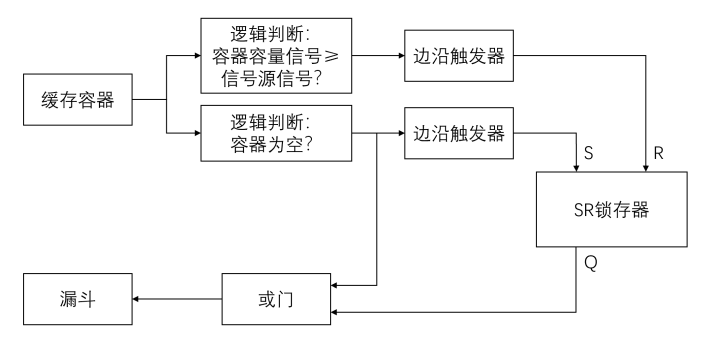
\includegraphics[width=.6\textwidth]{图1.png}
    \caption{工作原理示意图}
    \label{fig:1}
\end{figure}

{\bfseries 电路搭建:}按照图\ref{fig:1}所示工作原理,搭建实际电路如图\ref{fig:2}所示。其中各个组成部分具体说明如下:
\begin{enumerate}
    \item 比较器A:对容器进行容量检测,输出两个信号:将容器容量信号值传递给比较器C将“容器非空这一逻辑判断的结果传递给火把B。
    \item 火把B:非门,将“容器非空”取反当容器空时输出1,否则输出0。
    \item 比较器C:执行“容器容量信号大于等于信号源信号”这一逻辑判断。若将切换为减法模式,可以执行“严格大于”逻辑判断。
    \item 比较器D、蛋糕信号源,提供逻辑判断中用到的信号,详见说明。
    \item 两个投掷器:脸相对,内含一个物品构成SR锁存器。
    \item 观察者S边沿触发器,当火把B输出变化时,对SR锁存器进行置位。
    \item 观察者R:边沿触发器,当比较器C输出变化时,对SR锁存器进行复位。
    \item 比较器Q:SR锁存器的输出端。
    \item 红石粉、粘性活塞、红石块组成或门,当容器空或SR锁存器被置位时锁住漏斗,否则解锁漏斗。
\end{enumerate}

\begin{figure}[h]
    \centering
    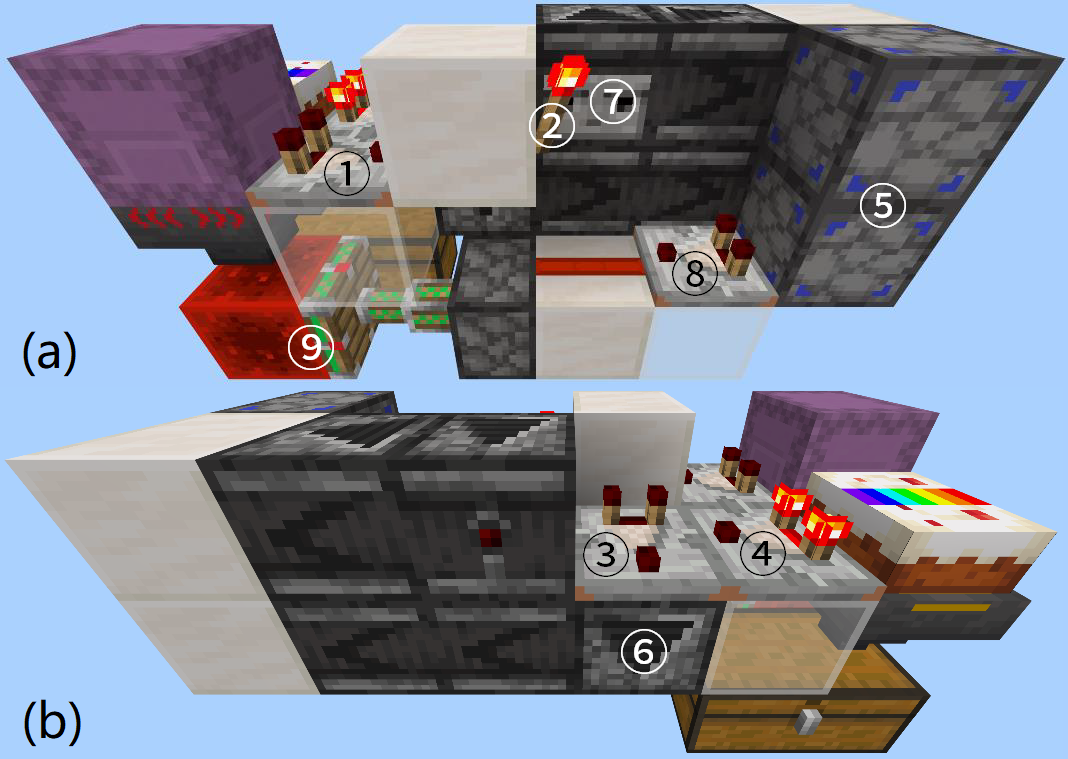
\includegraphics[width=.7\textwidth]{图2.png}
    \caption{实际电路图:(a)正面,(b)背面。}
    \label{fig:2}
\end{figure}

{\bfseries 运行过程分析:}
\begin{enumerate}
    \item 每一轮运行开始之前,缓存容器为空,SR锁存器处于置位状态,漏斗被锁定。
    \item 当容器被填入第一个物品时,火把B熄灭。锁存器收到置位信号,但由于已处于置位状态,故不发生其他改变。漏斗被锁定。
    \item 容器被逐渐填入物品。
    \item 当容器被填入物品数量足够多时,容量信号大于等于信号源信号,比较器C输出点亮,锁存器收到复位信号,变为复位状态。或门的两个输入现均为0,漏斗被解锁。
    \item 容器中被漏走一个(容器中有不同物品时,也可能数个)物品后,容量信号变为小于信号源信号,比较器C输出熄灭。锁存器收到复位信号,但由于已处于复位状态,故不发生其他改变。漏斗被解锁。
    \item 容器中的物品被逐渐漏走。
    \item 当容器中的最后一个物品被漏走时,火把B点亮,漏斗被锁定。同时,锁存器收到置位信号,变为置位状态。
    \item 等待下一轮运行开始。
\end{enumerate}

{\bfseries 运行过程分析:}

在本电路的工作环境中,判断“容器容量信号大于等于1”是无意义的,否则任一物品进入待检测容器后都会直接漏出,无法实现缓存功能。

使用1片蛋糕时,信号源提供强度为2的信号。若比较器C处于比较模式,则执行“大于等于2”的逻辑判断;若处于减法模式,则执行“严格大于2”的逻辑判断,等价于“大于等于3”。以此类推调整蛋糕的片数(从1到7)并切换比较器C的模式,即可实现“信号强度大于等于2/15”的判断。
\\

致谢:这种
物品缓存器的工作方式是由十室\footnote{B站用户名:地球人の实验室}提出的。感谢辰占鳌头\footnote{B站用户名:辰占鳌头}在本文写作过程中提供的大力支持。

\end{document}
